\subsection{The Split-Step Fourier method}
The Split-Step Fourier method can be used to solve nonlinear partial differential equations. The result is obtained by evolving the system in both the time and the frequency domain. Therefore the differential equation is split into a linear and a nonlinear part, which can be considered/regarded separately by using sufficiently small steps. The transformation between time and frequency domain can be achieved efficiently by a fast Fourier transform (FFT) algorithm, which makes this method desirable.

In order to solve the GPE we first take a look at the time-dependent Schr\"odinger equation (\ref{eqn:Schroedinger}).
In one spatial dimension its solution is
\begin{align}
\psi(z,t+\Delta t) = \exp\left[\alpha \left( -\frac{\hbar^2}{2m}\nabla^2 + V(z)\right) \right]\psi(z,t).
\end{align}
We defined $\displaystyle \alpha := -\frac i \hbar \Delta t $ simply for convenience.
Since the terms in the exponent do not commute, one cannot simply split the exponential function up. But if one rewrites the solution as
\begin{align}
\psi (z,t + \Delta t) = \exp\left(\frac \alpha 2 V(z)\right) \cdot 
\exp\left( -\alpha\frac{\hbar^2}{2m}\nabla^2\right) \cdot
\exp\left(\frac \alpha 2 V(z) \right) \cdot \psi(z,t),
\end{align}
the error is of $\mathcal{O}(\Delta t^3)$, which is accurate enough in our case and allows us to treat the two steps separately. Due to the fact, that $V$ is diagonal in the time domain and $\nabla^2$ is diagonal in the frequency domain, they simply become multiplications by $V(z)$ and the squared wavevector $k^2$, respectively. Combined with the speed of the FFT this enables a faster and more efficient way to obtain the result than calculating everything in the time domain would be.
Putting everything together yields
\begin{align}
\psi (z,t + \Delta t) = \exp\left(\frac \alpha 2 V(z)\right) \cdot \mathcal{F}^{-1} \left[
\exp\left( -\frac{\alpha\hbar^2}{2m}k^2\right) \cdot \mathcal{F} \left[
 \exp\left(\frac \alpha 2 V(z) \right) \cdot \psi(z,t) \right] \right].
\end{align}

Although we used the linear Schr\"odinger equation with time-independent Hamiltonian, the result is also true for the GPE if one replaces $V(x)$ by $V(x) + g\norm{\psi}^2$. By using the latest result in every step of the calculation one can ensure that the error does not exceed $\mathcal{O}(\Delta t^3)$.

Another important characteristic of the Split-Step Fourier method is, that it conserves the norm of the initial density distribution. To prove this for our implementation we normalized different initial constellations to 1 and plotted the norm after every time step during the evolution. The result is depicted in the following.
\begin{figure}[H]
	\centering
	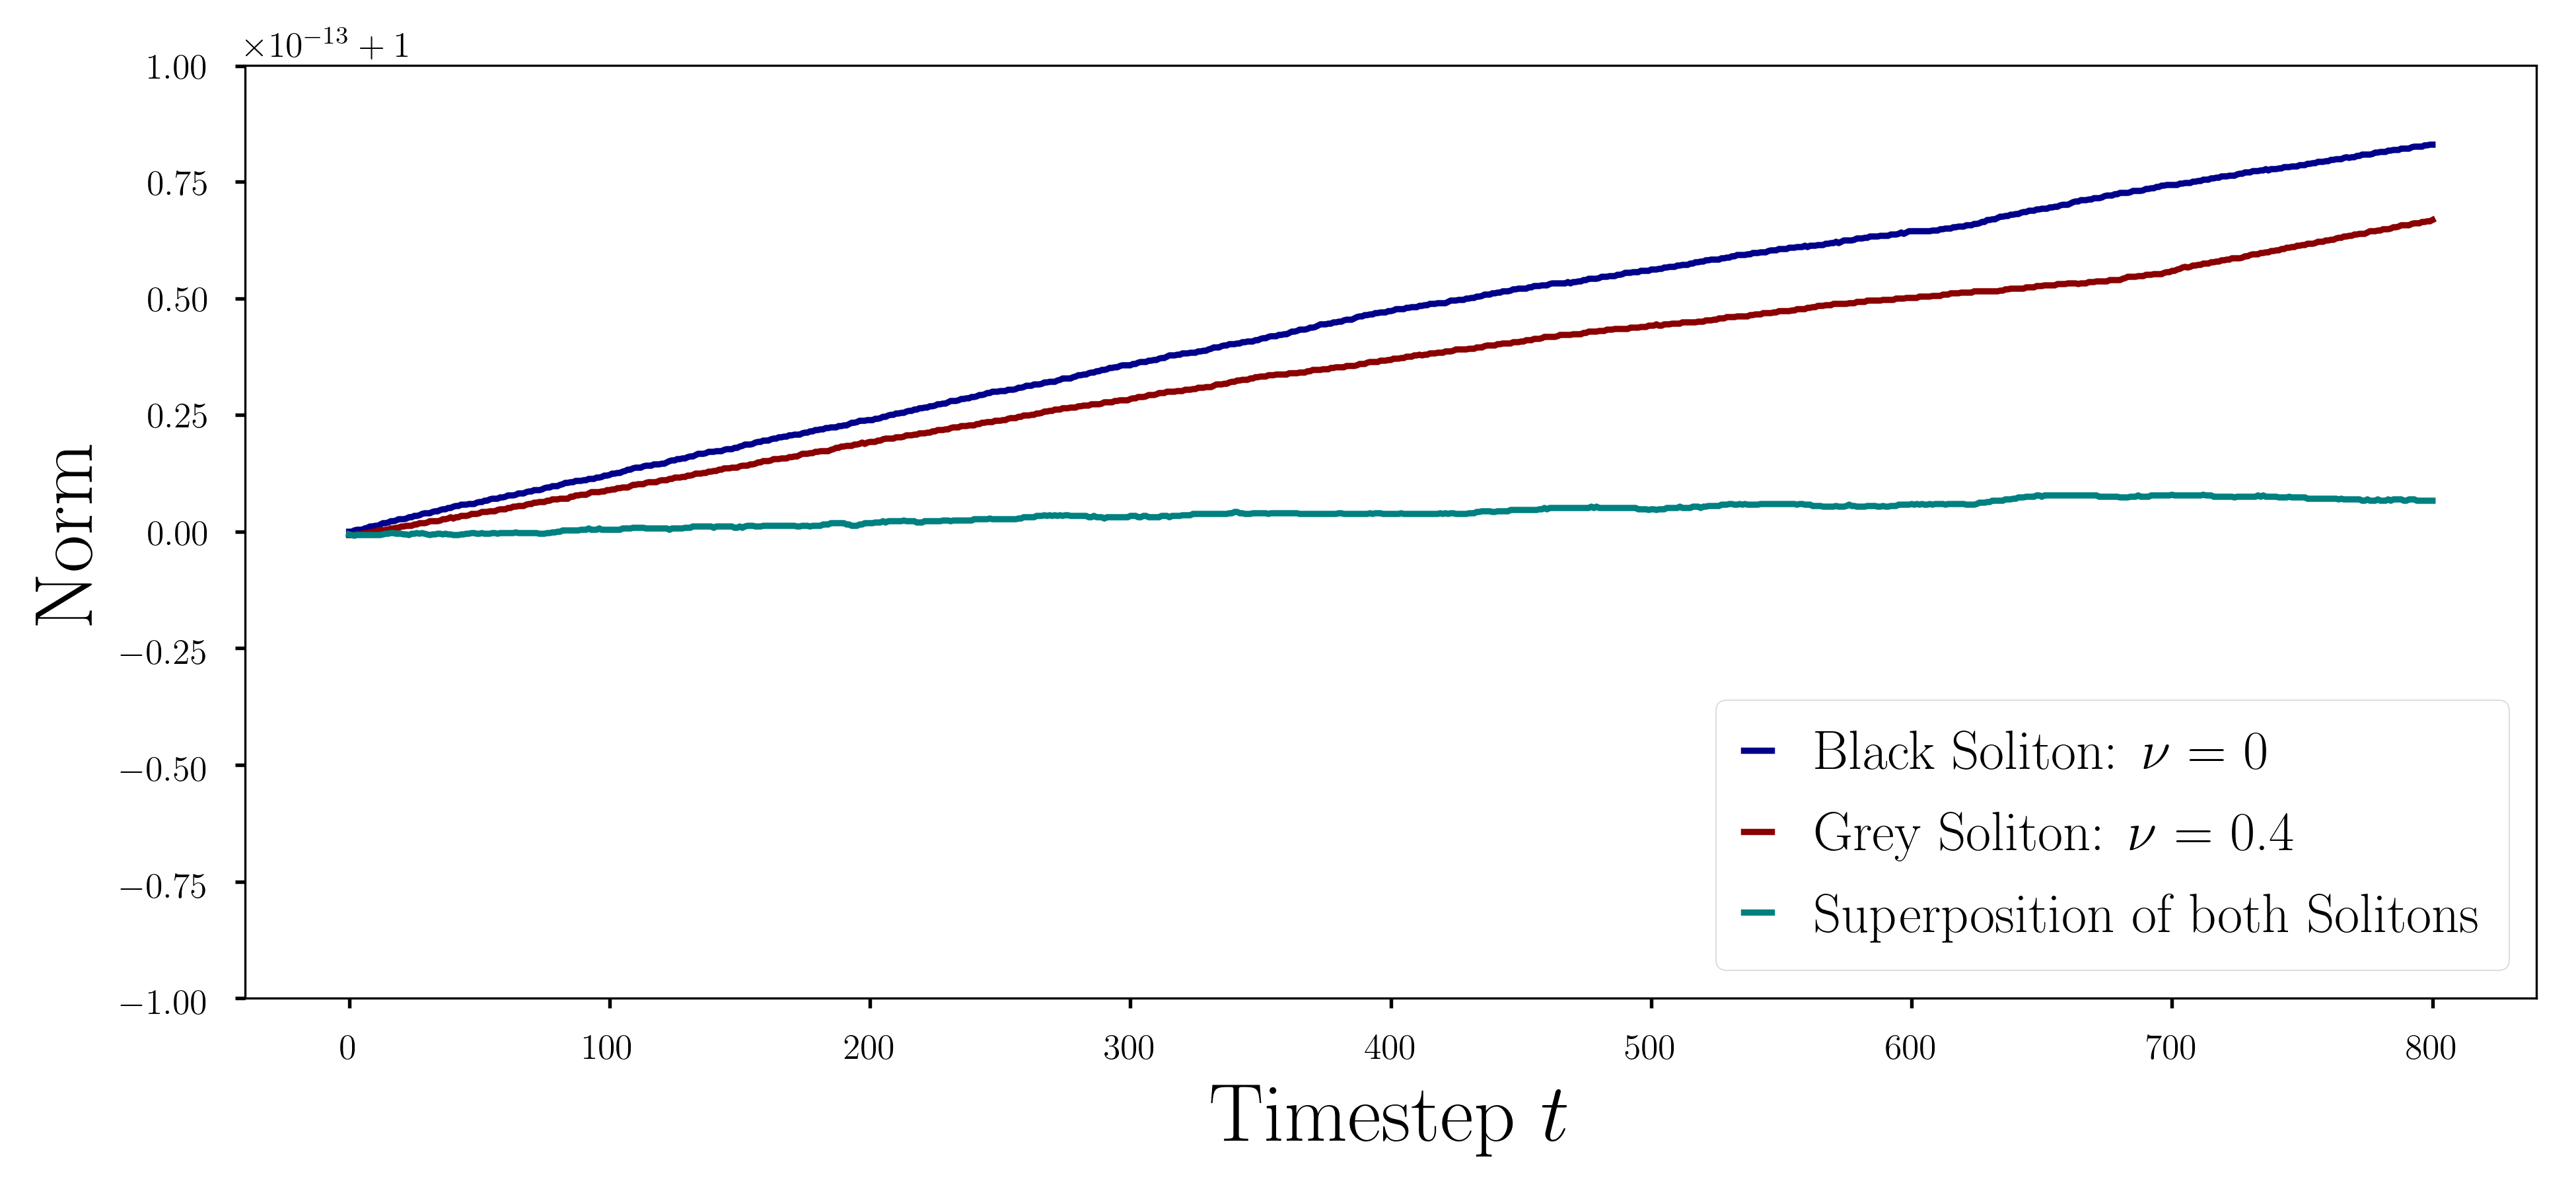
\includegraphics[scale = 0.25]{figures/norm}
	\caption{Proving the conservation of the norm by our implementation of the Split-Step Fourier method for different initial constellations.}
\end{figure}
As one can see, for our implementation the norm ist conserved within a limit of $\mathcal{O}(10^{-13})$.